% Chapter 12

\chapter{Análisis y Resultados} % Chapter title
\label{ch:analisis_resutados} % For referencing the chapter elsewhere, use \autoref{ch:name} 

El presente proyecto parte de la hipótesis de desarrollar una caché web distribuida que permita compartir de manera transparente y eficiente, los recursos computacionales distribuidos ofrecidos colaborativamente, mediante una comunidad de servidores. Se supone que ésto tendrá un impacto positivo en bajar los costos y en el mejoramiento de la continuidad del negocio para la comunidades virtuales. 

Dada la anterior hipótesis, se procedió a configurar los escenarios de pruebas descritos en la sección \ref{sec:escenarios}. Además se utilizó una configuración de hardware descrita en \ref{sec:parametros_pruebas}.

Como parte del proyecto se procedió con el desarrollo de un prototipo del protocolo CWC, el cual se describe en la sección \ref{sec:protitipo_cwc}.

La medición de las pruebas se realizó utilizando el software httperf y el software llamado time, mostrado en la sección \ref{subsec:time}. Creando un script que se encargara de medir la transmisión de los archivos definidos en la sección \ref{subsec:archivos} entre el cliente y el servidor, utilizando tanto el protocolo HTTP como el prototipo del protocolo CWC. 

%----------------------------------------------------------------------------------------
\section{Prototipo CWC}
\label{sec:protitipo_cwc}

El prototipo de CWC se programó utilizando el lenguaje de programación Python. Además se utilizó una biblioteca llamada btpeer. Ésta biblioteca implementa un protocolo P2P, el cual permite el intercambio de archivos. En la figura \ref{cwc} se pude ver la interfaz prototipo para un cliente-servidor.

\begin{figure}[h]
  \centering
    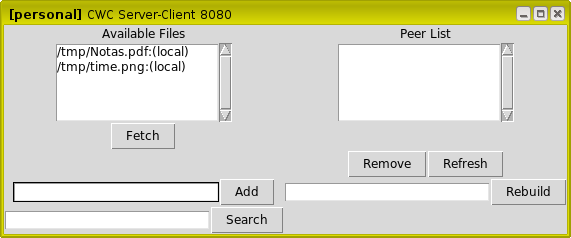
\includegraphics[scale=0.75]{gfx/cwc}
  \caption{Prototipo de CWC}
  \label{cwc}
\end{figure}

En el prototipo se centró en la transferencia de archivos a través de P2P, con el objetivo de realizar la comprobación de la hipótesis en cuanto a la transferencia eficiente y la baja en los costos de implementación de un sitio web. 

\section{Resultados de Rendimiento}
En la tabla \ref{tab:resultado_web} se detallan los resultados obtenidos cuando se ejecutó el escenario donde no existía Web Caché, en otras palabras en este escenario se configuró un servidor web, con los archivos descritos en la sección \ref{subsec:archivos} y se procedió a realizar la medición de tiempo de transferencia. Además como parte de la parametrización del escenario fue necesario limitar el ancho de banda a 200 KB/s utilizando la biblioteca de netfilter, con el utilitario iptables. Esta estrategia de limitación del ancho de banda fue definda en la sección \ref{subsec:estrategia_pruebas}.

\begin{table}[h] %here h, t top, b bottom, p dedicated page on floats
\myfloatalign
\begin{tabular}{lcccc} \toprule % four columns, fist left, other ones centered. 
\tableheadline{Tipo de Archivo} & \tableheadline{Tamaño (MB)} & \tableheadline{Servidor Web} \\ \midrule
Imágenes & 2.4 & 12.6 s \\ 
Videos & 345.9 & 1802.1 s  \\
Documentos & 1.3 & 6.6 s  \\
Instaladores & 34.6 & 181.2 s  \\
\end{tabular}
\caption{Resultados del escenario Sin Web Caché}  
\label{tab:resultado_web}
\end{table}

En la tabla \ref{tab:resultado_cwc} se documentó el resultado obtenido, luego de la ejecución del segundo escenario. En este escenario se utilizó el prototipo del protocolo CWC, donde se realizó la medición de la transferencia de datos de los archivos descritos en la sección \ref{subsec:archivos}, con el objetivo de compararlos con la tabla \ref{tab:resultado_web}. En este caso también se limitó el ancho de banda a 200 KB/s por nodo, como fue definido en las estrategias de pruebas de la sección \ref{subsec:estrategia_pruebas}.

\begin{table}[h] %here h, t top, b bottom, p dedicated page on floats
\myfloatalign
\begin{tabular}{lcccc} \toprule % four columns, fist left, other ones centered. 
\tableheadline{Tipo de Archivo} & \tableheadline{Tamaño (MB)} & \tableheadline{1 Nodo} & \tableheadline{2 nodos} & \tableheadline{3 nodos}\\ \midrule
Imágenes & 2.4  & 13.4 s & 12.9 s & 13.1 s \\ 
Videos & 345.9 & 1786.5 s &  902.8 s & 603.7 s \\
Documentos & 1.3 & 7.1 s & 6.9 s & 7.0 s \\
Instaladores & 34.6 & 168.4 s & 88.57 s & 58.2 s \\
\end{tabular}
\caption{Resultados del escenario Prototipo CWC}  
\label{tab:resultado_cwc}
\end{table}

\section{Análisis de rendimiento de velocidad del entorno de CWC}

Las herramientas seleccionadas para la medición del rendimiento fueron:
\begin{itemize}
\item Httperf: Se utilizó para medir el rendimiento del escenario Sin Web Caché
\item time: Se utilizó para medir el rendimiento del escenario del prototipo de CWC
\end{itemize}

Basado en la tabla \ref{tab:resultado_web} en combinación con la tabla \ref{tab:resultado_cwc} es posible concluir, que conforme más grande sea el archivo la red P2P, se comporta de una mejor manera. Por el contrario, esto no sucede con los archivos pequeños, pues estos archivos son servidos siempre desde un único nodo, según el protocolo. Por otro lado, se sirvieron archivos pequeños desde distintas ubicaciones, y ésto no significó mayor mejora, en cuanto al tiempo de respuesta. 

En la figura \ref{fig:respuesta_imagenes} se muestra la comparación de tiempo de transferencia de imágenes entre un servidor web con un nodo, en relación a la transferencia desde varios nodos, utilizando el protocolo CWC. No es posible comparar con varios servidores web, debido a que sin importar cuandos servidores web se agreguen, esto implicaría que el usuario siempre solo puede descargar el archivo desde una única ubicación. 

\begin{figure}[h!]
  \begin{center}    
\begin{tikzpicture}
  \centering
  \begin{axis}[
        ybar, axis on top,
        %title={Cumulative Progress of Works},
        height=8cm, width=\linewidth,
        bar width=0.4cm,
        ymajorgrids, tick align=inside,
        major grid style={draw=white},
        enlarge y limits={value=.1,upper},
        ymin=0, ymax=20,
        axis x line*=bottom,
        axis y line*=right,
        y axis line style={opacity=0},
        tickwidth=0pt,
        enlarge x limits=true,
        legend style={
            at={(0.5,-0.2)},
            anchor=north,
            legend columns=-1,
            /tikz/every even column/.append style={column sep=0.5cm}
        },
        ylabel={Tiempo (s)},
        symbolic x coords={
           HTTP,CWC-1 Nodo,CWC-2 Nodos,CWC-3 Nodos},
       xtick=data,
       nodes near coords={
        \pgfmathprintnumber[precision=0]{\pgfplotspointmeta}
       }
    ]
    \addplot [draw=none, fill=blue!30]
    table[x=servidor,y=tiempo,col sep=comma] {csv/imagenes.csv}; 

    %\legend{First Fix,Second Fix,Third Fix}
  \end{axis}
  \end{tikzpicture}
    
    \caption{Gráfico de tiempo de respuesta de imágenes.}
\label{fig:respuesta_imagenes}
  \end{center}
\end{figure}

Por otro lado, en la figura \ref{fig:respuesta_videos} se muestra la comparación de tiempo de transferencia de videos entre un servidor web con un nodo, en relación a la transferencia desde varios nodos, utilizando el protocolo CWC.


\begin{figure}[h!]
  \begin{center}    
\begin{tikzpicture}
  \centering
  \begin{axis}[
        ybar, axis on top,
        %title={Cumulative Progress of Works},
        height=8cm, width=\linewidth,
        bar width=0.4cm,
        ymajorgrids, tick align=inside,
        major grid style={draw=white},
        enlarge y limits={value=.1,upper},
        ymin=0, ymax=2000,
        axis x line*=bottom,
        axis y line*=right,
        y axis line style={opacity=0},
        tickwidth=0pt,
        enlarge x limits=true,
        legend style={
            at={(0.5,-0.2)},
            anchor=north,
            legend columns=-1,
            /tikz/every even column/.append style={column sep=0.5cm}
        },
        ylabel={Tiempo (s)},
        symbolic x coords={
           HTTP,CWC-1 Nodo,CWC-2 Nodos,CWC-3 Nodos},
       xtick=data,
       nodes near coords={
        \pgfmathprintnumber[precision=0]{\pgfplotspointmeta}
       }
    ]
    \addplot [draw=none, fill=blue!30]
    table[x=servidor,y=tiempo,col sep=comma] {csv/videos.csv}; 

    %\legend{First Fix,Second Fix,Third Fix}
  \end{axis}
  \end{tikzpicture}
    
    \caption{Gráfico de tiempo de respuesta de videos.}
\label{fig:respuesta_videos}
  \end{center}
\end{figure}

Siguiendo con el mismo ejercicio, en la figura \ref{fig:respuesta_documentos} se muestra la comparación de tiempo de transferencia de documentos entre un servidor web con un nodo, en relación a la transferencia desde varios nodos, utilizando el protocolo CWC.

\begin{figure}[h!]
  \begin{center}    
\begin{tikzpicture}
  \centering
  \begin{axis}[
        ybar, axis on top,
        %title={Cumulative Progress of Works},
        height=8cm, width=\linewidth,
        bar width=0.4cm,
        ymajorgrids, tick align=inside,
        major grid style={draw=white},
        enlarge y limits={value=.1,upper},
        ymin=0, ymax=10,
        axis x line*=bottom,
        axis y line*=right,
        y axis line style={opacity=0},
        tickwidth=0pt,
        enlarge x limits=true,
        legend style={
            at={(0.5,-0.2)},
            anchor=north,
            legend columns=-1,
            /tikz/every even column/.append style={column sep=0.5cm}
        },
        ylabel={Tiempo (s)},
        symbolic x coords={
           HTTP,CWC-1 Nodo,CWC-2 Nodos,CWC-3 Nodos},
       xtick=data,
       nodes near coords={
        \pgfmathprintnumber[precision=0]{\pgfplotspointmeta}
       }
    ]
    \addplot [draw=none, fill=blue!30]
    table[x=servidor,y=tiempo,col sep=comma] {csv/documentos.csv}; 

    %\legend{First Fix,Second Fix,Third Fix}
  \end{axis}
  \end{tikzpicture}
    
    \caption{Gráfico de tiempo de respuesta de documentos.}
      \label{fig:respuesta_documentos}
  \end{center}
\end{figure}

Y por último, en la figura \ref{fig:respuesta_instaladores} se muestra la comparación de tiempo de transferencia de instaladores entre un servidor web con un nodo, en relación a la transferencia desde varios nodos, utilizando el protocolo CWC.

\begin{figure}[h!]
  \begin{center}    
\begin{tikzpicture}
  \centering
  \begin{axis}[
        ybar, axis on top,
        %title={Cumulative Progress of Works},
        height=8cm, width=\linewidth,
        bar width=0.4cm,
        ymajorgrids, tick align=inside,
        major grid style={draw=white},
        enlarge y limits={value=.1,upper},
        ymin=0, ymax=200,
        axis x line*=bottom,
        axis y line*=right,
        y axis line style={opacity=0},
        tickwidth=0pt,
        enlarge x limits=true,
        legend style={
            at={(0.5,-0.2)},
            anchor=north,
            legend columns=-1,
            /tikz/every even column/.append style={column sep=0.5cm}
        },
        ylabel={Tiempo (s)},
        symbolic x coords={
           HTTP,CWC-1 Nodo,CWC-2 Nodos,CWC-3 Nodos},
       xtick=data,
       nodes near coords={
        \pgfmathprintnumber[precision=0]{\pgfplotspointmeta}
       }
    ]
    \addplot [draw=none, fill=blue!30]
    table[x=servidor,y=tiempo,col sep=comma] {csv/instaladores.csv}; 

    %\legend{First Fix,Second Fix,Third Fix}
  \end{axis}
  \end{tikzpicture}
    
    \caption{Gráfico de tiempo de respuesta de instaladores.}
  \label{fig:respuesta_instaladores}
  \end{center}
\end{figure}

Dado este resultado, es fácil comprobar la hipótesis que el protocolo CWC utiliza eficientemente los recursos computacionales en comparación con un modelo tradicional de cliente-servidor, el cual se encuentra representado por el protocolo HTTP. 

\section{Resultados de Costo}
Como parte del análisis de costos fue necesario realizar una compilación de precios estándares de mercado, basados en la configuración de hardware presente en la sección \ref{subsec:servidor_web}. Los precios fueron tomados de uno de los sitios más utilizados para la compra de artículos en la web, el mismo es Amazon \cite{amazon:cpu, amazon:hd, amazon:memoria, amazon:network}. En la tabla \ref{tab:resultado_costo} se muestra la comparación de costos entre un servidor web y la configuración del prototipo CWC con varias configuraciones en cuanto a tamaño de nodos. 

\begin{table}[h] %here h, t top, b bottom, p dedicated page on floats
\myfloatalign
\begin{tabular}{lcccc} \toprule % four columns, fist left, other ones centered. 
\tableheadline{Componente} & \tableheadline{Servidor Web} & \tableheadline{1 Nodo} & \tableheadline{2 nodos} & \tableheadline{3 nodos}\\ \midrule
Memoria & \$40  & \$40  & \$0 & \$0 \\ 
Procesador & \$120 & \$120 & \$0 & \$0 \\
Almacenamiento & \$55 & \$55 & \$0 & \$0 \\
Interfaz de Red & \$10 & \$40 & \$0 & \$0 \\
Total & \$255 & \$255 & \$0 & \$0 \\
\end{tabular}
\caption{Comparación de costos}  
\label{tab:resultado_costo}
\end{table}


%----------------------------------------------------------------------------------------

\section{Análisis de costos del Entorno de CW}

En el caso del CWC, basado en la tabla \ref{tab:resultado_costo}, es posible determinar que entre más nodos más barato es el mantenimiento del sitio. Esto pues, los nodos adicionales se componen de recursos que son cedidos a través de la comunidad. Por otro lado, también se puede concluir basado en la tabla \ref{tab:resultado_cwc} y la tabla \ref{tab:resultado_costo} que el costo decrece, y el servicio aumenta, si aumentamos el número de nodos conectados a la comunidad. 

Por otro lado, en la figura \ref{fig:comparacion_costos} se puede observar que el costo de la infraestructura utilizando el protocolo CWC es constante, si se incrementan la cantidad de nodos en la red. Mientras que los costos utilizando el protocolo HTTP tienden al alza. 

\begin{figure}[h!]
  \begin{center}    
\begin{tikzpicture}
  \begin{axis}[
  	width=\linewidth, % Scale the plot to \linewidth
    grid=major, % Display a grid
    grid style={dashed,gray!30}, % Set the style
    legend style={at={(0.5,-0.2)},anchor=north},
    x tick label style={rotate=90,anchor=east},
    xmin = 1, xmax = 4,
    ymin = 0, ymax = 1100,
    axis y line* = left, % the '*' avoids arrow heads
    xlabel = Cantidad de Servidores,
    ylabel = Costo(\$)]
    \addplot[red]
    table[x=nodos,y=costo http,col sep=comma] {csv/costos.csv}; 
    \legend{Costo de HTTP}
  \end{axis}
  \begin{axis}[
	width=\linewidth, % Scale the plot to \linewidth
	legend style={at={(0.5,-0.3)},anchor=north},
    xmin = 1, xmax = 4,
    ymin = 0, ymax = 1100,
    hide x axis,
    hide y axis]
    \addplot[blue]
    table[x=nodos,y=costo cwc,col sep=comma] {csv/costos.csv}; 
    \legend{Costo de CWC}
  \end{axis}
  \pgfplotsset{every axis y label/.append style={rotate=180,yshift=9.5cm}}
  \begin{axis}[
  		width=\linewidth, % Scale the plot to \linewidth
        xmin=1, xmax=4,
        ymin=0, ymax=1100,
        hide x axis,
        axis y line*=right,
        ylabel={Teste es el otro}
    ]
  \end{axis}
\end{tikzpicture}
    
    \caption{Gráfico de comparación de costos.}
  \label{fig:comparacion_costos}
  \end{center}
\end{figure}

Dada la anterior conclusión, se puede comprobar que el protocolo CWC utilizando los recursos computacionales aportados por una comunidad tiene un impacto positivo en bajar los costos al momento de realizar una publicación en Internet. 

\section{Análisis de continuidad de negocio y transparencia}
Basado en la figura \ref{fig:respuesta_instaladores}, se puede observar que conforme se agreguen más nodos al sistema de CWC, se mejora el tiempo de atención de los clientes. Por otro lado si incrementáramos la cantidad de servidores HTTP, esto no sucedería. 

El agregar más servidores HTTP como espejo, aunque sí implica una mejora en la continuidad del negocio, impactaría en los costos de administración e implicaría la necesidad de utilizar protocolos adicionales como el DNS o un balanceo de cargas, para asegurar esta misma continuidad. 

Eliminar servidores HTTP de continuidad de negocio también implica cambios en la configuración del DNS o de los balanceadores y este cambio tiende a no ser transparente. Por el contrario, el agregar miembros a la comunidad CWC es una acción que ya se encuentra contemplada en el mismo protocolo. 	

Dado el análisis anterior, se muestra que el protocolo CWC mejora la administración de la continuidad del negocio, haciendo éste proceso más fácil y transparente para el administrador del sitio web. 